\documentclass[11pt]{article}

\usepackage[margin=1in]{geometry}
\usepackage[T1]{fontenc}
\usepackage[utf8]{inputenc}
\usepackage{lmodern}
\usepackage{microtype}
\usepackage{amsmath,amssymb,amsthm,mathtools}
\usepackage{bm}
\usepackage{booktabs,array,longtable}
\usepackage{hyperref}
\usepackage{xcolor}
\usepackage[most]{tcolorbox}
\usepackage{tikz}
\usepackage{pgfplots}
\usepackage{pgfplotstable}
\usepackage{tikz-3dplot}
\usepackage{enumitem}
\usepackage{caption}
\usepackage{float}
\usepackage{fancyhdr}
\usepackage{titlesec}

\pgfplotsset{compat=1.18}
\usetikzlibrary{arrows.meta,calc,intersections,patterns,decorations.pathreplacing,positioning,3d,backgrounds}

\hypersetup{
  colorlinks=true,
  linkcolor=blue!60!black,
  urlcolor=blue!60!black,
  citecolor=blue!60!black,
  pdftitle={Chapter 12. Constrained Optimization and Lagrange Multipliers}
}

\setlength{\headheight}{14pt}
\setlength{\parindent}{0pt}
\setlength{\parskip}{0.65em}
\setlist[itemize]{topsep=2pt,itemsep=2pt}
\setlist[enumerate]{topsep=2pt,itemsep=2pt}

\titleformat{\section}{\large\bfseries}{\thesection}{0.6em}{}
\titleformat{\subsection}{\normalsize\bfseries}{\thesubsection}{0.6em}{}

\pagestyle{fancy}
\fancyhf{}
\lhead{Chapter 12. Constrained Optimization and Lagrange Multipliers}
\rhead{\thepage}
\renewcommand{\headrulewidth}{0.4pt}

\newtcolorbox{chapteroverviewbox}{
  colback=blue!4,
  colframe=blue!50!black,
  boxrule=0.7pt,
  arc=2mm,
  left=2mm,right=2mm,top=1mm,bottom=1mm
}

\newtcolorbox{goalbox}{
  colback=green!4,
  colframe=green!45!black,
  title=Learning objectives,
  fonttitle=\bfseries,
  boxrule=0.7pt,
  arc=2mm
}

\newtcolorbox{tipbox}[1][]{
  colback=green!3,
  colframe=green!45!black,
  title=#1,
  fonttitle=\bfseries,
  boxrule=0.7pt,
  arc=2mm
}

\newtcolorbox{notebox}[1][]{
  colback=blue!3,
  colframe=blue!50!black,
  title=#1,
  fonttitle=\bfseries,
  boxrule=0.7pt,
  arc=2mm
}

\newtcolorbox{importantbox}[1][]{
  colback=red!3,
  colframe=red!60!black,
  title=#1,
  fonttitle=\bfseries,
  boxrule=0.7pt,
  arc=2mm
}

\newtcolorbox{warningbox}[1][]{
  colback=yellow!8,
  colframe=orange!75!black,
  title=#1,
  fonttitle=\bfseries,
  boxrule=0.7pt,
  arc=2mm
}

\newtcbtheorem[number within=section]{workedexample}{Worked example}{
  enhanced,
  breakable,
  colback=white,
  colframe=blue!60!black,
  colbacktitle=blue!60!black,
  fonttitle=\bfseries,
  boxrule=0.7pt,
  arc=1.5mm,
  left=2mm,right=2mm,top=1mm,bottom=1mm
}{ex}

\newcommand{\R}{\mathbb R}
\newcommand{\grad}{\nabla}
\newcommand{\dd}{\,d}
\newcommand{\norm}[1]{\left\lVert #1\right\rVert}

\begin{document}

\begin{center}
  {\LARGE\bfseries Chapter 12. Constrained Optimization and Lagrange Multipliers\par}
  \vspace{0.3em}
  {\large Optimizing under equations, budgets, geometry, and model constraints\par}
\end{center}

\begin{chapteroverviewbox}
Many important optimization problems are not free optimization problems. A model may need to satisfy a budget, a probability vector must have total mass $1$, a point may be required to lie on a curve or surface, and a physical system may preserve mass or energy. This chapter develops the method of Lagrange multipliers, a geometric and computational tool for optimizing a function subject to one or more constraints.

In unconstrained optimization, an interior local maximum or minimum of a differentiable function usually satisfies $\grad f=0$. Constrained optimization is different. If the point must stay on a curve such as $x^2+y^2=10$, the variables cannot move independently. At an optimal constrained point, a level curve of $f$ is tangent to the constraint curve. Equivalently, the normal vectors are parallel.
\end{chapteroverviewbox}

\begin{goalbox}
After studying this chapter, you should be able to:
\begin{enumerate}
  \item distinguish unconstrained and constrained optimization problems;
  \item explain the geometric meaning of the condition $\grad f=\lambda \grad g$;
  \item solve constrained optimization problems with one equality constraint;
  \item combine interior critical points with boundary candidates for absolute extrema;
  \item solve distance, area, volume, and budget problems using constraints;
  \item use Lagrange multipliers with two equality constraints;
  \item recognize when the method needs regularity assumptions such as $\grad g\ne 0$;
  \item interpret constrained optimization in statistics, machine learning, and applied mathematics.
\end{enumerate}
\end{goalbox}

\section{What makes an optimization problem constrained?}

A typical unconstrained optimization problem asks for the maximum or minimum of $f(x,y)$ over a region where $(x,y)$ can move freely. A constrained optimization problem asks for the maximum or minimum of $f(x,y)$ subject to an equation such as
\[
g(x,y)=k.
\]
The function $f$ is the \emph{objective function}. The equation $g(x,y)=k$ is the \emph{constraint}. The set of all points satisfying the constraint is the \emph{constraint set}.

For example,
\[
f(x,y)=2x+6y,\qquad x^2+y^2=10
\]
asks us to optimize a linear function along a circle. We are not allowed to move anywhere in the plane; we may only move along the circle.

\begin{tipbox}[The optimization question has two parts]
Every constrained optimization problem should be read as:
\begin{enumerate}
  \item \textbf{Objective:} What quantity are we trying to maximize or minimize?
  \item \textbf{Constraint:} What equations or restrictions must the variables satisfy?
\end{enumerate}
Most mistakes come from confusing the objective with the constraint.
\end{tipbox}

\section{The geometry of tangency}

Suppose $f(x,y)$ is to be optimized subject to $g(x,y)=k$. The constraint is a level curve of $g$. The objective also has level curves $f(x,y)=c$.

At a constrained maximum or minimum, the level curve of $f$ usually just touches the constraint curve. If the two curves crossed transversely, then moving along the constraint would move $f$ both upward and downward, so the point would not be an extremum.

Gradients are normal to level curves. Therefore, at a regular constrained extremum,
\[
\grad f \quad \text{is parallel to} \quad \grad g.
\]
This means that there is a scalar $\lambda$ such that
\[
\grad f=\lambda \grad g.
\]
The number $\lambda$ is called a \emph{Lagrange multiplier}.

\begin{figure}[H]
\centering
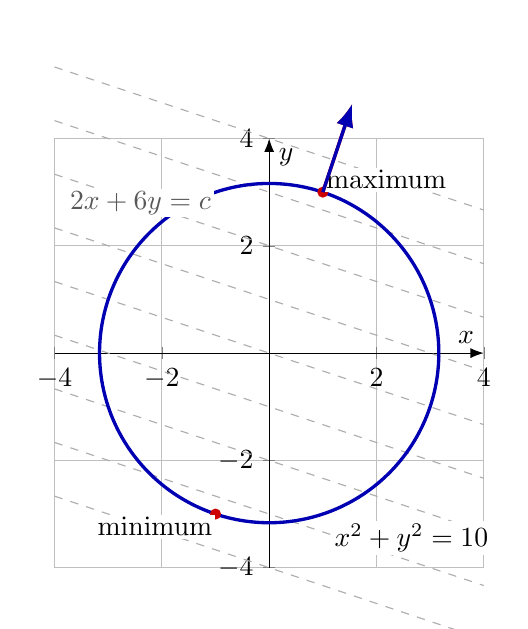
\begin{tikzpicture}
\begin{axis}[
  width=0.72\textwidth,
  height=0.58\textwidth,
  xmin=-4,xmax=4,
  ymin=-4,ymax=4,
  axis equal image,
  axis lines=middle,
  xlabel={$x$},ylabel={$y$},
  grid=both,
  axis line style={-Latex},
  clip=false
]
\foreach \c in {-24,-18,-12,-6,0,6,12,18,24}{
  \addplot[domain=-4:4,samples=2,gray!65,dashed] {(\c-2*x)/6};
}
\addplot[domain=0:360,samples=250,very thick,blue!70!black] ({sqrt(10)*cos(x)},{sqrt(10)*sin(x)});
\fill[red!80!black] (axis cs:1,3) circle (2pt);
\fill[red!80!black] (axis cs:-1,-3) circle (2pt);
\node[above right,fill=white,inner sep=1pt] at (axis cs:1,3) {maximum};
\node[below left,fill=white,inner sep=1pt] at (axis cs:-1,-3) {minimum};
\addplot[red!80!black,very thick,-Latex] coordinates {(1,3) (1.55,4.65)};
\addplot[blue!70!black,very thick,-Latex] coordinates {(1,3) (1.55,4.65)};
\node[fill=white,inner sep=1pt] at (axis cs:2.65,-3.45) {$x^2+y^2=10$};
\node[gray!70!black,fill=white,inner sep=1pt] at (axis cs:-2.4,2.8) {$2x+6y=c$};
\end{axis}
\end{tikzpicture}
\caption{At a constrained extremum, a level curve of the objective is tangent to the constraint curve. The normal directions are parallel.}
\end{figure}

\section{The method of Lagrange multipliers: one constraint}

Let $f$ and $g$ be differentiable functions of $x$ and $y$. To find extrema of $f(x,y)$ subject to $g(x,y)=k$, solve the system
\[
\grad f(x,y)=\lambda \grad g(x,y),\qquad g(x,y)=k.
\]
Equivalently,
\[
\begin{cases}
f_x=\lambda g_x,\\
f_y=\lambda g_y,\\
g(x,y)=k.
\end{cases}
\]
For a function of three variables subject to one constraint $g(x,y,z)=k$, solve
\[
\begin{cases}
f_x=\lambda g_x,\\
f_y=\lambda g_y,\\
f_z=\lambda g_z,\\
g(x,y,z)=k.
\end{cases}
\]

\begin{importantbox}[Regularity assumption]
The standard Lagrange multiplier condition assumes that the constraint is regular at the point, meaning $\grad g\ne 0$. If $\grad g=0$ somewhere on the constraint set, the method may miss an extremum or produce incomplete information. Such points must be checked separately.
\end{importantbox}

\begin{notebox}[Algorithm: equality-constrained extrema]
To optimize $f$ subject to $g=k$:
\begin{enumerate}
  \item Compute $\grad f$ and $\grad g$.
  \item Set up $\grad f=\lambda \grad g$ together with $g=k$.
  \item Solve for the variables and $\lambda$.
  \item Evaluate $f$ at all candidate points.
  \item If the constraint set is closed and bounded and $f$ is continuous, the largest value is the absolute maximum and the smallest value is the absolute minimum.
\end{enumerate}
\end{notebox}

\section{A first worked example: a linear objective on a circle}

\begin{workedexample}{A linear objective on a circle}{linear-circle}
Find the maximum and minimum values of
\[
f(x,y)=2x+6y
\]
subject to $x^2+y^2=10$.

Let $g(x,y)=x^2+y^2$. Then
\[
\grad f=\langle 2,6\rangle,
\qquad
\grad g=\langle 2x,2y\rangle.
\]
The Lagrange equations are
\[
\langle 2,6\rangle=\lambda\langle 2x,2y\rangle,
\qquad x^2+y^2=10.
\]
Thus
\[
2=2\lambda x,\qquad 6=2\lambda y.
\]
Assuming $\lambda\ne 0$,
\[
x=\frac1\lambda,\qquad y=\frac3\lambda.
\]
Substitution into the constraint gives
\[
\frac{1}{\lambda^2}+\frac{9}{\lambda^2}=10,
\]
so $\lambda^2=1$. Therefore $\lambda=1$ gives $(x,y)=(1,3)$, while $\lambda=-1$ gives $(x,y)=(-1,-3)$. Since
\[
f(1,3)=20,\qquad f(-1,-3)=-20,
\]
the maximum value is $20$ and the minimum value is $-20$.
\end{workedexample}

\begin{figure}[H]
\centering
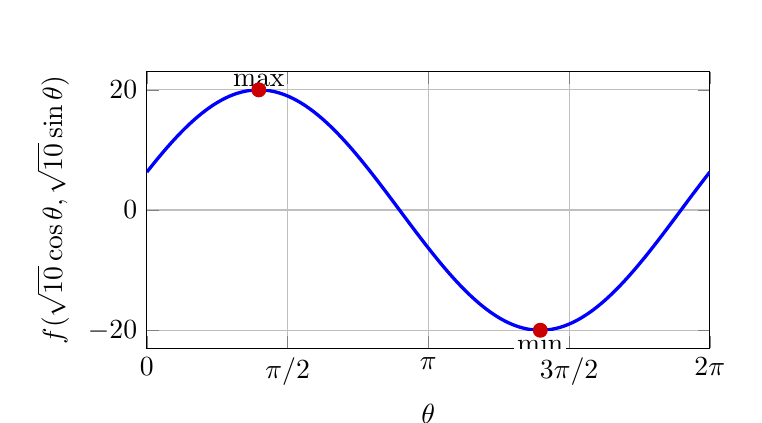
\begin{tikzpicture}
\begin{axis}[
  width=0.72\textwidth,
  height=0.42\textwidth,
  xmin=0,xmax=6.283,
  ymin=-23,ymax=23,
  xlabel={$\theta$},
  ylabel={$f(\sqrt{10}\cos\theta,\sqrt{10}\sin\theta)$},
  grid=both,
  xtick={0,1.5708,3.1416,4.7124,6.283},
  xticklabels={$0$,$\pi/2$,$\pi$,$3\pi/2$,$2\pi$}
]
\addplot[very thick,blue,domain=0:6.283,samples=300] {2*sqrt(10)*cos(deg(x)) + 6*sqrt(10)*sin(deg(x))};
\addplot[only marks,mark=*,mark size=2.5pt,red!80!black] coordinates {(1.249,20) (4.391,-20)};
\node[above,fill=white,inner sep=1pt] at (axis cs:1.249,20) {max};
\node[below,fill=white,inner sep=1pt] at (axis cs:4.391,-20) {min};
\end{axis}
\end{tikzpicture}
\caption{The objective restricted to the circle becomes a one-variable function of the angle $\theta$.}
\end{figure}

\section{Why $\grad f=\lambda \grad g$ means no feasible first-order change}

Suppose $r(t)$ is a path that stays on the constraint set, so $g(r(t))=k$. Differentiating gives
\[
\grad g(r(t))\cdot r'(t)=0.
\]
Thus the velocity vector $r'(t)$ is tangent to the constraint set. At a constrained extremum, $f(r(t))$ should have derivative zero for every feasible tangent direction:
\[
\frac{\dd}{\dd t}f(r(t))=\grad f(r(t))\cdot r'(t)=0.
\]
So $\grad f$ must be perpendicular to every tangent direction. But $\grad g$ is also perpendicular to every tangent direction. Therefore, in the one-constraint case, $\grad f$ and $\grad g$ must be parallel.

\section{Distance problems}

Distance problems are among the cleanest applications of Lagrange multipliers.

\begin{workedexample}{Closest point on a parabola}{closest-parabola}
Find the point on $y=x^2$ closest to $(0,1)$.

Minimize the squared distance
\[
f(x,y)=x^2+(y-1)^2
\]
subject to
\[
g(x,y)=y-x^2=0.
\]
The gradients are
\[
\grad f=\langle 2x,2(y-1)\rangle,
\qquad
\grad g=\langle -2x,1\rangle.
\]
The Lagrange equations are
\[
\begin{cases}
2x=-2\lambda x,\\
2(y-1)=\lambda,\\
y=x^2.
\end{cases}
\]
The first equation gives $x(1+\lambda)=0$. If $x=0$, then $y=0$. If $\lambda=-1$, then $2(y-1)=-1$, so $y=1/2$ and hence $x=\pm 1/\sqrt2$.

The candidate points are
\[
(0,0),\qquad \left(\frac1{\sqrt2},\frac12\right),\qquad \left(-\frac1{\sqrt2},\frac12\right).
\]
Since
\[
f(0,0)=1,
\qquad
f\left(\pm\frac1{\sqrt2},\frac12\right)=\frac34,
\]
the closest points are
\[
\left(\frac1{\sqrt2},\frac12\right)
\quad\text{and}\quad
\left(-\frac1{\sqrt2},\frac12\right).
\]
\end{workedexample}

\begin{figure}[H]
\centering
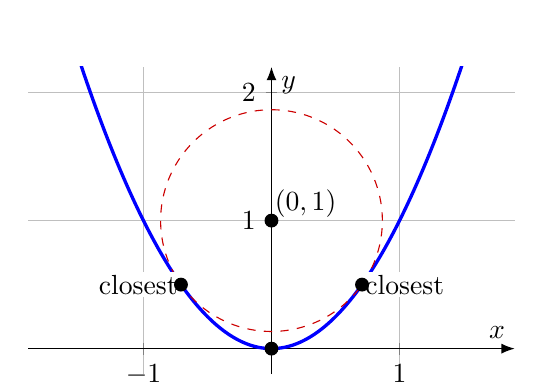
\begin{tikzpicture}
\begin{axis}[
  width=0.64\textwidth,
  height=0.58\textwidth,
  xmin=-1.9,xmax=1.9,
  ymin=-0.2,ymax=2.2,
  axis equal image,
  axis lines=middle,
  xlabel={$x$},ylabel={$y$},
  grid=both,
  axis line style={-Latex}
]
\addplot[domain=-1.75:1.75,samples=250,very thick,blue] {x^2};
\addplot[domain=0:360,samples=250,red!80!black,dashed] ({(sqrt(3)/2)*cos(x)},{1+(sqrt(3)/2)*sin(x)});
\addplot[only marks,mark=*,mark size=2.3pt] coordinates {(0,1) (0,0) (0.7071,0.5) (-0.7071,0.5)};
\node[above right,fill=white,inner sep=1pt] at (axis cs:0,1) {$(0,1)$};
\node[right,fill=white,inner sep=1pt] at (axis cs:0.7071,0.5) {closest};
\node[left,fill=white,inner sep=1pt] at (axis cs:-0.7071,0.5) {closest};
\end{axis}
\end{tikzpicture}
\caption{The closest points occur where a distance circle centered at $(0,1)$ is tangent to the parabola.}
\end{figure}

\section{Absolute extrema on closed bounded regions}

For a closed bounded region $D$, absolute extrema of a continuous function $f$ can occur:
\begin{enumerate}
  \item at interior critical points, where $\grad f=0$;
  \item on smooth boundary pieces, where Lagrange multipliers apply;
  \item at corners or nonsmooth boundary points.
\end{enumerate}

\begin{notebox}[Interior-boundary-corner checklist]
To find absolute maxima and minima on a closed bounded region:
\begin{enumerate}
  \item Find all interior critical points.
  \item Analyze each boundary piece.
  \item Use Lagrange multipliers on curved or implicit boundary pieces.
  \item Check corners and endpoints.
  \item Evaluate $f$ at every candidate.
\end{enumerate}
\end{notebox}

\begin{workedexample}{A quadratic function on a disk}{disk-extrema}
Find the maximum and minimum of
\[
f(x,y)=x^2+2y^2+2
\]
on the disk $D=\{(x,y):x^2+y^2\le 1\}$.

Interior critical points satisfy
\[
\grad f=\langle 2x,4y\rangle=0,
\]
so the only interior critical point is $(0,0)$, where $f(0,0)=2$.

On the boundary $x^2+y^2=1$, let $g(x,y)=x^2+y^2$. The Lagrange equations are
\[
\langle 2x,4y\rangle=\lambda\langle 2x,2y\rangle,
\qquad x^2+y^2=1.
\]
The boundary candidates are $(\pm1,0)$ and $(0,\pm1)$. Evaluating,
\[
f(\pm1,0)=3,
\qquad
f(0,\pm1)=4,
\qquad
f(0,0)=2.
\]
Therefore, the absolute minimum is $2$ at $(0,0)$, and the absolute maximum is $4$ at $(0,\pm1)$.
\end{workedexample}

\begin{figure}[H]
\centering
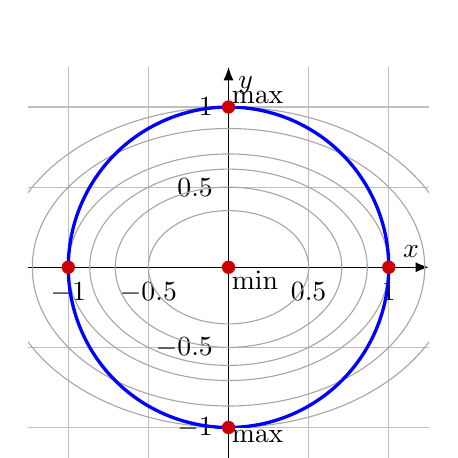
\begin{tikzpicture}
\begin{axis}[
  width=0.6\textwidth,
  height=0.55\textwidth,
  xmin=-1.25,xmax=1.25,
  ymin=-1.25,ymax=1.25,
  axis equal image,
  axis lines=middle,
  xlabel={$x$},ylabel={$y$},
  grid=both,
  axis line style={-Latex}
]
\foreach \c in {0.25,0.5,0.75,1.0,1.5,2.0}{
  \addplot[domain=0:360,samples=220,gray!70] ({sqrt(\c)*cos(x)},{sqrt(\c/2)*sin(x)});
}
\addplot[domain=0:360,samples=250,very thick,blue] ({cos(x)},{sin(x)});
\addplot[only marks,mark=*,mark size=2.2pt,red!80!black] coordinates {(0,0) (1,0) (-1,0) (0,1) (0,-1)};
\node[below right,fill=white,inner sep=1pt] at (axis cs:0,0) {min};
\node[above right,fill=white,inner sep=1pt] at (axis cs:0,1) {max};
\node[below right,fill=white,inner sep=1pt] at (axis cs:0,-1) {max};
\end{axis}
\end{tikzpicture}
\caption{Absolute extrema on a disk require checking both the interior and the boundary.}
\end{figure}

\section{Area and volume under constraints}

Many modeling problems involve maximizing or minimizing a geometric quantity while preserving a resource.

\begin{workedexample}{Maximum area with fixed perimeter}{max-area}
A rectangle has perimeter $12$. Find the dimensions that maximize its area.

Let $x$ and $y$ be side lengths. The area is $A(x,y)=xy$. The perimeter constraint is $2x+2y=12$. Compute
\[
\grad A=\langle y,x\rangle,
\qquad
\grad g=\langle 2,2\rangle.
\]
The Lagrange equations give
\[
\langle y,x\rangle=\lambda\langle 2,2\rangle,
\qquad 2x+2y=12.
\]
Thus $y=2\lambda$ and $x=2\lambda$, so $x=y$. From $2x+2y=12$, we get $x=y=3$. The maximum-area rectangle is a square of side length $3$, and the maximum area is $9$.
\end{workedexample}

\begin{figure}[H]
\centering
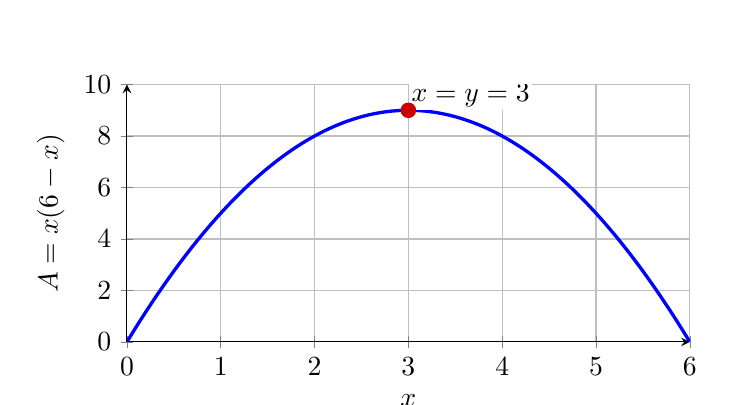
\begin{tikzpicture}
\begin{axis}[
  width=0.72\textwidth,
  height=0.40\textwidth,
  xmin=0,xmax=6,
  ymin=0,ymax=10,
  xlabel={$x$},ylabel={$A=x(6-x)$},
  grid=both,
  axis lines=left
]
\addplot[domain=0:6,samples=250,very thick,blue] {x*(6-x)};
\addplot[only marks,mark=*,mark size=2.6pt,red!80!black] coordinates {(3,9)};
\node[above right,fill=white,inner sep=1pt] at (axis cs:3,9) {$x=y=3$};
\end{axis}
\end{tikzpicture}
\caption{With fixed perimeter $12$, the rectangle area $xy$ is maximized when $x=y=3$.}
\end{figure}

\begin{workedexample}{Minimizing material for a box with fixed volume}{box-volume}
A box with no top has volume $4$. Find the dimensions that minimize the cardboard area.

Let $x$, $y$, and $z$ be the length, width, and height. The volume constraint is $xyz=4$, and the cardboard area is
\[
A(x,y,z)=xy+2xz+2yz.
\]
Solving the constraint for $z$ gives $z=4/(xy)$. Hence
\[
A(x,y)=xy+\frac8y+\frac8x.
\]
Set partial derivatives equal to zero:
\[
A_x=y-\frac8{x^2}=0,
\qquad
A_y=x-\frac8{y^2}=0.
\]
By symmetry, $x=y$. Then $x=8/x^2$, so $x^3=8$ and $x=2$. Thus $y=2$, and the volume constraint gives $z=1$. The minimal cardboard dimensions are $2\times2\times1$.
\end{workedexample}

\section{Lagrange multipliers in three variables}

For one constraint in three variables, the method is exactly the same:
\[
\grad f(x,y,z)=\lambda \grad g(x,y,z),
\qquad g(x,y,z)=k.
\]

\begin{workedexample}{Closest point on a plane}{plane-projection}
Find the point on the plane $2x+y-z=1$ closest to $(0,1,3)$.

Minimize squared distance
\[
f(x,y,z)=x^2+(y-1)^2+(z-3)^2
\]
subject to $g(x,y,z)=2x+y-z=1$. Then
\[
\grad f=\langle 2x,2(y-1),2(z-3)\rangle,
\qquad
\grad g=\langle 2,1,-1\rangle.
\]
The Lagrange equations give
\[
2x=2\lambda,
\qquad
2(y-1)=\lambda,
\qquad
2(z-3)=-\lambda.
\]
Thus
\[
x=\lambda,
\qquad
 y=1+\frac\lambda2,
\qquad
 z=3-\frac\lambda2.
\]
Substitution into $2x+y-z=1$ gives $3\lambda-2=1$, so $\lambda=1$. Therefore,
\[
(x,y,z)=\left(1,\frac32,\frac52\right).
\]
\end{workedexample}

\begin{figure}[H]
\centering
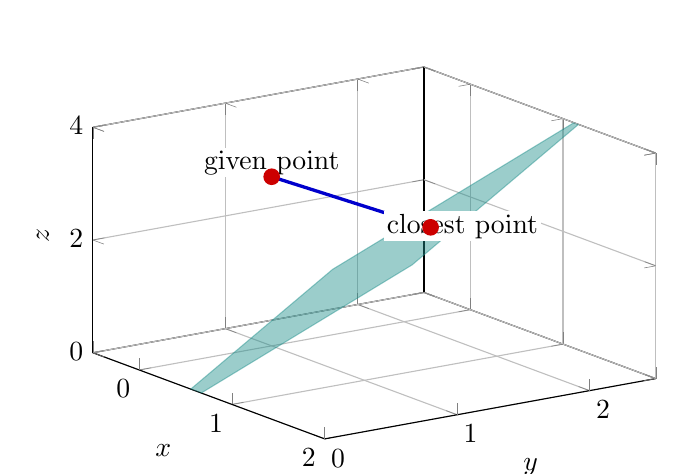
\begin{tikzpicture}
\begin{axis}[
  width=0.72\textwidth,
  height=0.52\textwidth,
  view={55}{25},
  xlabel={$x$},ylabel={$y$},zlabel={$z$},
  xmin=-0.5,xmax=2,
  ymin=0,ymax=2.5,
  zmin=0,zmax=4,
  grid=major,
  colormap/viridis
]
\addplot3[surf,shader=flat,opacity=0.45,domain=-0.2:1.8,y domain=0.2:2.2,samples=2,samples y=2] {2*x+y-1};
\addplot3[only marks,mark=*,mark size=2.8pt,red!80!black] coordinates {(0,1,3) (1,1.5,2.5)};
\addplot3[very thick,blue!80!black] coordinates {(0,1,3) (1,1.5,2.5)};
\node[fill=white,inner sep=1pt] at (axis cs:0,1,3.25) {given point};
\node[fill=white,inner sep=1pt] at (axis cs:1.2,1.6,2.6) {closest point};
\end{axis}
\end{tikzpicture}
\caption{The closest point on a plane is obtained by moving from the given point in the normal direction.}
\end{figure}

\section{Hot and cold spots in a solid ball}

Constrained optimization is often combined with interior optimization. Suppose the temperature in a solid ball of radius $2$ is
\[
T(x,y,z)=x^2+y^2+2z^2-2x+2y.
\]
The solid ball is $x^2+y^2+z^2\le 4$. To find the hottest and coldest spots, check:
\begin{enumerate}
  \item interior critical points, where $\grad T=0$;
  \item boundary points on the sphere $x^2+y^2+z^2=4$.
\end{enumerate}
Interior critical points satisfy
\[
\grad T=\langle 2x-2,2y+2,4z\rangle=0,
\]
so the interior critical point is $(1,-1,0)$, and it lies inside the ball because $1^2+(-1)^2+0^2=2<4$.

On the boundary, solve
\[
\begin{cases}
2x-2=2\lambda x,\\
2y+2=2\lambda y,\\
4z=2\lambda z,\\
x^2+y^2+z^2=4.
\end{cases}
\]
This illustrates a common feature of three-variable Lagrange multiplier problems: algebra may split into cases. The method gives candidate points; then we evaluate the temperature at all candidates and compare.

\begin{figure}[H]
\centering
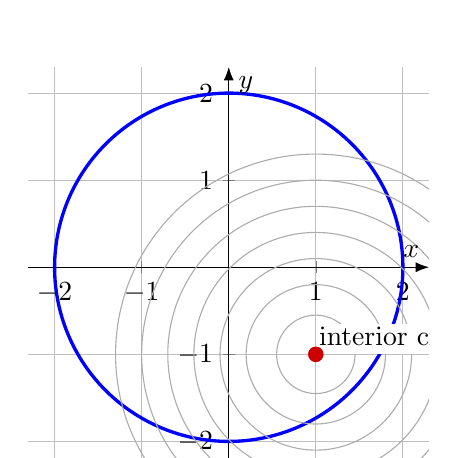
\begin{tikzpicture}
\begin{axis}[
  width=0.62\textwidth,
  height=0.55\textwidth,
  xmin=-2.3,xmax=2.3,
  ymin=-2.3,ymax=2.3,
  axis equal image,
  axis lines=middle,
  xlabel={$x$},ylabel={$y$},
  grid=both,
  axis line style={-Latex}
]
\addplot[domain=0:360,samples=250,very thick,blue] ({2*cos(x)},{2*sin(x)});
\foreach \r in {0.45,0.8,1.1,1.4,1.7,2.0,2.3}{
  \addplot[domain=0:360,samples=200,gray!65] ({1+\r*cos(x)},{-1+\r*sin(x)});
}
\addplot[only marks,mark=*,mark size=2.6pt,red!80!black] coordinates {(1,-1)};
\node[above right,fill=white,inner sep=1pt] at (axis cs:1,-1) {interior critical point};
\end{axis}
\end{tikzpicture}
\caption{A slice $z=0$ of the temperature field. The disk boundary and interior critical point must both be checked.}
\end{figure}

\section{Multiple constraints}

Suppose $f(x,y,z)$ is to be optimized subject to two constraints:
\[
g(x,y,z)=k,
\qquad
h(x,y,z)=c.
\]
The constraint set is often a curve in space: the intersection of two surfaces. At a regular constrained extremum, $\grad f$ is perpendicular to the tangent direction of the constraint curve. The gradients $\grad g$ and $\grad h$ are also perpendicular to that tangent direction. Therefore,
\[
\grad f=\lambda \grad g+\mu \grad h.
\]
The system is
\[
\begin{cases}
f_x=\lambda g_x+\mu h_x,\\
f_y=\lambda g_y+\mu h_y,\\
f_z=\lambda g_z+\mu h_z,\\
g(x,y,z)=k,\\
h(x,y,z)=c.
\end{cases}
\]

\begin{notebox}[Geometric meaning of two constraints]
With one constraint in $\R^3$, the feasible set is usually a surface. With two constraints in $\R^3$, the feasible set is usually a curve. At an extremum on that curve, $\grad f$ must be orthogonal to the curve's tangent direction, so it must be a linear combination of the two constraint normals.
\end{notebox}

\begin{workedexample}{Two constraints}{two-constraints}
Find the extreme values of
\[
f(x,y,z)=xy+yz
\]
subject to
\[
xy=1,
\qquad y^2+z^2=9.
\]
Let $g(x,y,z)=xy$ and $h(x,y,z)=y^2+z^2$. Then
\[
\grad f=\langle y,x+z,y\rangle,
\qquad
\grad g=\langle y,x,0\rangle,
\qquad
\grad h=\langle 0,2y,2z\rangle.
\]
The constraints give $x=1/y$ and $z^2=9-y^2$, so on the constraint set,
\[
f=xy+yz=1+yz.
\]
Since $y^2+z^2=9$, the product $yz$ lies between $-9/2$ and $9/2$. Therefore
\[
f_{\max}=1+\frac92=\frac{11}{2},
\qquad
f_{\min}=1-\frac92=-\frac72.
\]
The corresponding points are obtained from $x=1/y$ and the sign choices for $y$ and $z$.
\end{workedexample}

\begin{figure}[H]
\centering
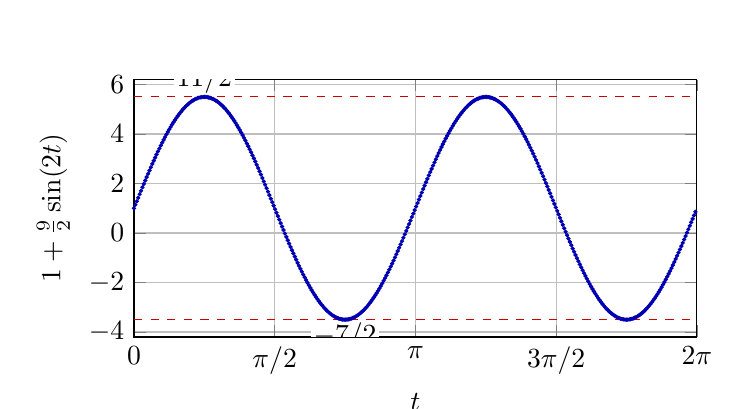
\begin{tikzpicture}
\begin{axis}[
  width=0.72\textwidth,
  height=0.40\textwidth,
  xmin=0,xmax=6.283,
  ymin=-4.2,ymax=6.2,
  xlabel={$t$},ylabel={$1+\frac{9}{2}\sin(2t)$},
  grid=both,
  xtick={0,1.5708,3.1416,4.7124,6.283},
  xticklabels={$0$,$\pi/2$,$\pi$,$3\pi/2$,$2\pi$}
]
\addplot[domain=0:6.283,samples=400,only marks,mark=*,mark size=0.55pt,blue!70!black] {1+4.5*sin(deg(2*x))};
\addplot[red!80!black,dashed] coordinates {(0,5.5) (6.283,5.5)};
\addplot[red!80!black,dashed] coordinates {(0,-3.5) (6.283,-3.5)};
\node[above,fill=white,inner sep=1pt] at (axis cs:0.785,5.5) {$11/2$};
\node[below,fill=white,inner sep=1pt] at (axis cs:2.356,-3.5) {$-7/2$};
\end{axis}
\end{tikzpicture}
\caption{With two constraints, the feasible set can be parameterized; the objective varies along the feasible curve.}
\end{figure}

\section{Lagrange multipliers and machine learning constraints}

Many machine-learning and statistics problems are constrained optimization problems.

\subsection*{Probability simplex}
A probability vector $p=(p_1,\dots,p_n)$ must satisfy
\[
p_i\ge 0,
\qquad
\sum_{i=1}^n p_i=1.
\]
The equality constraint is $g(p)=\sum_i p_i=1$. When maximizing entropy
\[
H(p)=-\sum_{i=1}^n p_i\log p_i
\]
subject to $\sum_i p_i=1$, the Lagrange multiplier equation leads to the uniform distribution when there are no additional constraints.

\subsection*{Normalized parameters}
Some models impose a normalization constraint such as $\norm{w}^2=1$. Optimizing a quadratic form
\[
f(w)=w^T A w
\]
subject to $w^T w=1$ leads to
\[
Aw=\lambda w,
\]
which is an eigenvalue problem. This is one reason eigenvectors appear naturally in principal component analysis, spectral methods, and constrained variance maximization.

\subsection*{Regularization versus hard constraints}
A constrained problem might look like
\[
\min_w L(w)\quad \text{subject to}\quad \norm{w}^2\le c.
\]
A related unconstrained problem is
\[
\min_w L(w)+\alpha \norm{w}^2.
\]
The constrained version uses a hard budget on model complexity. The regularized version uses a penalty. Lagrange multipliers explain why these two viewpoints are closely related.

\begin{figure}[H]
\centering
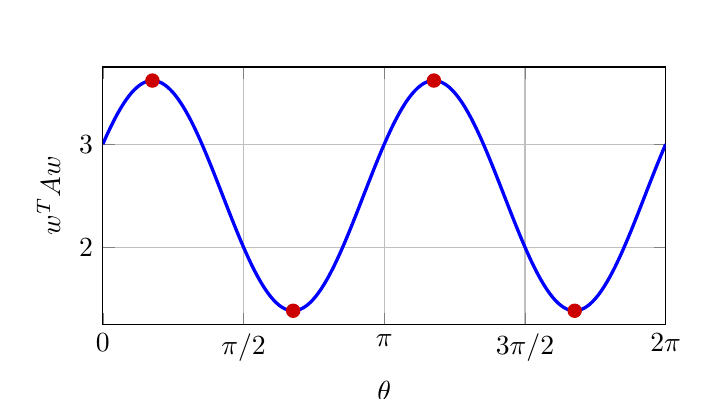
\begin{tikzpicture}
\begin{axis}[
  width=0.72\textwidth,
  height=0.40\textwidth,
  xmin=0,xmax=6.283,
  ymin=1.25,ymax=3.75,
  xlabel={$\theta$},ylabel={$w^T A w$},
  grid=both,
  xtick={0,1.5708,3.1416,4.7124,6.283},
  xticklabels={$0$,$\pi/2$,$\pi$,$3\pi/2$,$2\pi$}
]
\addplot[domain=0:6.283,samples=400,very thick,blue] {3*cos(deg(x))^2 + 2*sin(deg(x))^2 + 2*sin(deg(x))*cos(deg(x))};
\addplot[only marks,mark=*,mark size=2.4pt,red!80!black] coordinates {(0.554,3.618) (3.696,3.618) (2.125,1.382) (5.267,1.382)};
\end{axis}
\end{tikzpicture}
\caption{Optimizing a quadratic form on the unit circle leads to eigenvector directions.}
\end{figure}

\section{Numerical search on a constraint}

Even when exact algebra is difficult, the geometry remains useful. A curve constraint can often be parameterized, sampled, or solved numerically.

For example, consider
\[
f(x,y)=x^2-xy+2y^2
\]
on the ellipse
\[
\frac{x^2}{4}+y^2=1.
\]
A parameterization is
\[
x=2\cos t,
\qquad y=\sin t.
\]
Then the constrained problem becomes the one-variable problem
\[
F(t)=f(2\cos t,\sin t).
\]
This parameterization method does not replace Lagrange multipliers, but it is an excellent way to check answers and build intuition.

\begin{figure}[H]
\centering
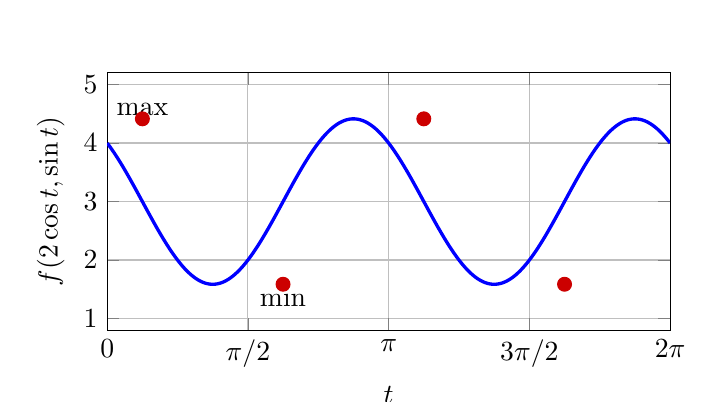
\begin{tikzpicture}
\begin{axis}[
  width=0.72\textwidth,
  height=0.40\textwidth,
  xmin=0,xmax=6.283,
  ymin=0.8,ymax=5.2,
  xlabel={$t$},ylabel={$f(2\cos t,\sin t)$},
  grid=both,
  xtick={0,1.5708,3.1416,4.7124,6.283},
  xticklabels={$0$,$\pi/2$,$\pi$,$3\pi/2$,$2\pi$}
]
\addplot[domain=0:6.283,samples=400,very thick,blue] {4*cos(deg(x))^2 - 2*cos(deg(x))*sin(deg(x)) + 2*sin(deg(x))^2};
\addplot[only marks,mark=*,mark size=2.5pt,red!80!black] coordinates {(0.393,4.414) (3.534,4.414) (1.963,1.586) (5.105,1.586)};
\node[above,fill=white,inner sep=1pt] at (axis cs:0.393,4.414) {max};
\node[below,fill=white,inner sep=1pt] at (axis cs:1.963,1.586) {min};
\end{axis}
\end{tikzpicture}
\caption{A constrained problem can be checked numerically by parameterizing the constraint.}
\end{figure}

\section{When Lagrange multipliers may fail or need care}

The equation $\grad f=\lambda \grad g$ is powerful, but it is not magic. It requires a smooth constraint and a nonzero constraint gradient.

Be careful in the following situations:
\begin{enumerate}
  \item \textbf{The constraint gradient vanishes.} If $\grad g=0$ at a feasible point, check that point separately.
  \item \textbf{The constraint has corners or cusps.} A nonsmooth boundary may not have a well-defined normal vector.
  \item \textbf{The feasible set is not closed or not bounded.} Absolute extrema may fail to exist.
  \item \textbf{The constraint is an inequality.} Lagrange multipliers handle equality constraints directly. Inequality constraints require checking interiors, active boundaries, and sometimes more advanced conditions.
  \item \textbf{Solving the equations gives candidates, not conclusions.} Always evaluate the objective and compare values when looking for absolute extrema.
\end{enumerate}

\begin{warningbox}[Candidate points are not automatically extrema]
Solving the Lagrange equations gives possible constrained extrema. It does not automatically classify them. For absolute extrema, evaluate $f$ at all candidates and compare values. For local classification, additional second-order constrained tests or local analysis may be needed.
\end{warningbox}

\section{Summary}

The central idea of constrained optimization is that variables are not free to move in all directions. At an optimal feasible point, all allowable first-order changes fail to increase or decrease the objective in the relevant direction.

For one equality constraint $g(x)=k$, the condition is
\[
\grad f=\lambda \grad g.
\]
For two equality constraints in three variables,
\[
g(x,y,z)=k,
\qquad h(x,y,z)=c,
\]
the condition is
\[
\grad f=\lambda \grad g+\mu \grad h.
\]
The method is used across mathematics, statistics, economics, physics, engineering, machine learning, and artificial intelligence. It explains why optimum solutions often occur where level sets are tangent, why normalization constraints lead to eigenvalue problems, and why penalties and constraints are two sides of the same modeling idea.

\section{Exercises}

\subsection*{Conceptual exercises}
\begin{enumerate}
  \item Explain why $\grad f=0$ is not usually true at a constrained maximum or minimum.
  \item Draw a picture showing why the level curve of $f$ should be tangent to the constraint curve $g=k$ at a constrained extremum.
  \item What does the condition $\grad g\ne 0$ mean geometrically?
  \item In a closed disk, why must one check both interior critical points and the boundary?
  \item Explain the difference between a hard constraint and a penalty term in an optimization problem.
\end{enumerate}

\subsection*{Computational exercises}
\begin{enumerate}[start=6]
  \item Use Lagrange multipliers to find the maximum and minimum of $f(x,y)=x+2y$ subject to $x^2+y^2=5$.
  \item Use Lagrange multipliers to find the maximum and minimum of $f(x,y)=xy$ subject to $x^2+y^2=8$.
  \item Find the point on the line $3x+4y=12$ closest to the origin.
  \item Find the point on the plane $x+y+z=1$ closest to $(2,0,0)$.
  \item Find the maximum area of a rectangle with perimeter $20$.
  \item Find the dimensions of a closed rectangular box of volume $64$ with minimum surface area.
  \item Find the maximum and minimum of $f(x,y)=x^2+4y^2$ on the circle $x^2+y^2=1$.
  \item Find the maximum and minimum of $f(x,y)=x^2+y^2$ subject to $x+2y=4$.
  \item Find the constrained critical points of $f(x,y)=x^3+y^2$ subject to $3x+2y=0$.
  \item Find the closest point on the parabola $y=x^2$ to the point $(0,2)$.
\end{enumerate}

\subsection*{Applied and computational exercises}
\begin{enumerate}[start=16]
  \item A company has a budget constraint $4L+9K=360$, where $L$ is labor and $K$ is capital. Suppose production is $P(L,K)=L^{1/2}K^{1/2}$. Use Lagrange multipliers to maximize production.
  \item A probability vector $(p_1,p_2,p_3)$ satisfies $p_1+p_2+p_3=1$ and $p_i>0$. Use Lagrange multipliers to maximize $H(p)=-\sum p_i\log p_i$.
  \item Maximize $w^T A w$ subject to $w^T w=1$ for $A=\begin{pmatrix}2&0\\0&5\end{pmatrix}$. Interpret the answer geometrically.
  \item A cylindrical can has fixed volume $V$. Use constrained optimization to find the radius and height that minimize surface area.
  \item A point must lie on the sphere $x^2+y^2+z^2=9$. Find the maximum and minimum of $f(x,y,z)=x+2y+2z$.
  \item Numerically parameterize the circle $x^2+y^2=10$ and confirm the extrema of $f(x,y)=2x+6y$.
  \item Parameterize the ellipse $x^2/9+y^2/4=1$ and numerically optimize $f(x,y)=xy$.
  \item Use a grid search on the unit disk to approximate the maximum and minimum of $f(x,y)=x^2+2y^2+2$. Compare with the exact solution.
\end{enumerate}

\end{document}
